

\tikzset{every picture/.style={line width=0.75pt}} %set default line width to 0.75pt        

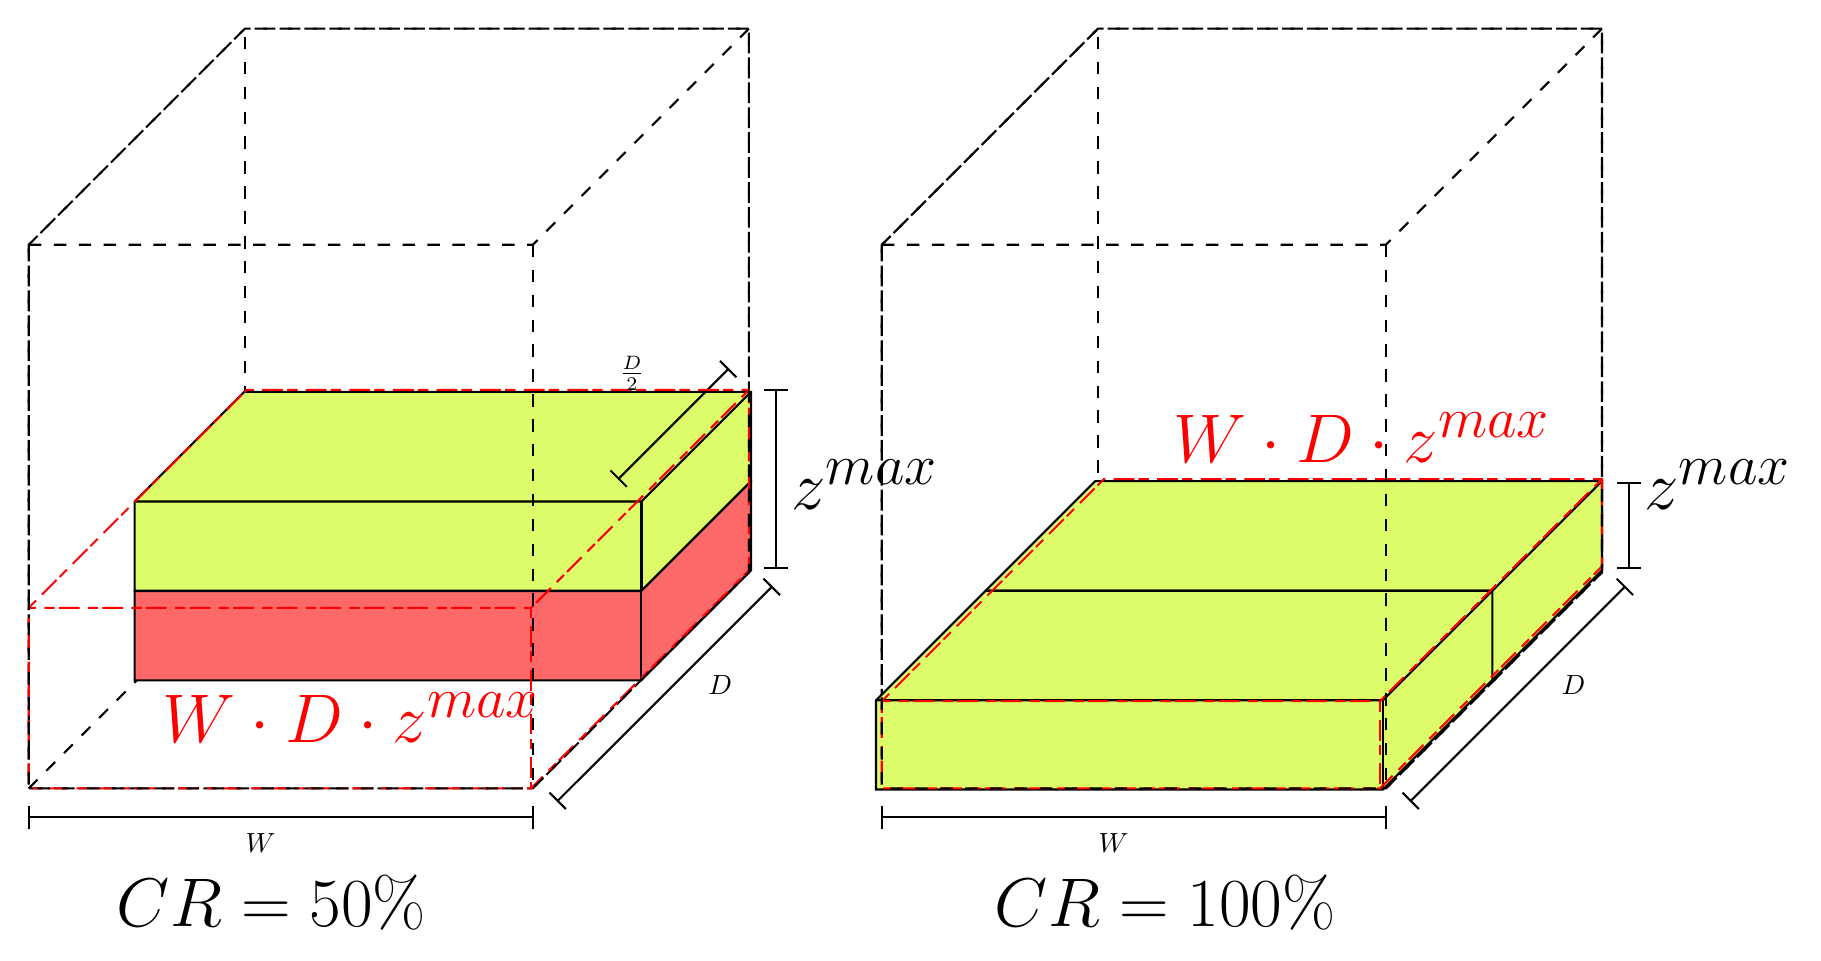
\begin{tikzpicture}[x=0.75pt,y=0.75pt,yscale=-1,xscale=1]
%uncomment if require: \path (0,479); %set diagram left start at 0, and has height of 479

%Shape: Cube [id:dp9446615397697055] 
\draw  [dash pattern={on 4.5pt off 4.5pt}] (917,301.9) -- (812.9,406) -- (570,406) -- (570,144.1) -- (674.1,40) -- (917,40) -- cycle ; \draw  [dash pattern={on 4.5pt off 4.5pt}] (570,406) -- (674.1,301.9) -- (917,301.9) ; \draw  [dash pattern={on 4.5pt off 4.5pt}] (674.1,301.9) -- (674.1,40) ;
%Shape: Cube [id:dp9924623151681093] 
\draw  [fill={rgb, 255:red, 220; green, 253; blue, 105 }  ,fill opacity=1 ] (620,310.78) -- (672.78,258) -- (917,258) -- (917,301) -- (864.22,353.78) -- (620,353.78) -- cycle ; \draw   (917,258) -- (864.22,310.78) -- (620,310.78) ; \draw   (864.22,310.78) -- (864.22,353.78) ;
%Shape: Cube [id:dp4356357707795666] 
\draw  [fill={rgb, 255:red, 220; green, 253; blue, 105 }  ,fill opacity=1 ] (567.22,363.56) -- (620,310.78) -- (864.22,310.78) -- (864.22,353.78) -- (811.44,406.56) -- (567.22,406.56) -- cycle ; \draw   (864.22,310.78) -- (811.44,363.56) -- (567.22,363.56) ; \draw   (811.44,363.56) -- (811.44,406.56) ;
%Shape: Cube [id:dp900981008021689] 
\draw  [dash pattern={on 4.5pt off 4.5pt}] (506,301.9) -- (401.9,406) -- (159,406) -- (159,144.1) -- (263.1,40) -- (506,40) -- cycle ; \draw  [dash pattern={on 4.5pt off 4.5pt}] (159,406) -- (263.1,301.9) -- (506,301.9) ; \draw  [dash pattern={on 4.5pt off 4.5pt}] (263.1,301.9) -- (263.1,40) ;
%Shape: Cube [id:dp9462720863667783] 
\draw  [fill={rgb, 255:red, 253; green, 105; blue, 105 }  ,fill opacity=1 ] (210,311) -- (263,258) -- (507,258) -- (507,301) -- (454,354) -- (210,354) -- cycle ; \draw   (507,258) -- (454,311) -- (210,311) ; \draw   (454,311) -- (454,354) ;
%Shape: Cube [id:dp20686523528460465] 
\draw  [fill={rgb, 255:red, 220; green, 253; blue, 105 }  ,fill opacity=1 ] (210,267.78) -- (262.78,215) -- (507,215) -- (507,258) -- (454.22,310.78) -- (210,310.78) -- cycle ; \draw   (507,215) -- (454.22,267.78) -- (210,267.78) ; \draw   (454.22,267.78) -- (454.22,310.78) ;
%Straight Lines [id:da9583369995131138] 
\draw    (496,204) -- (443.22,256.78) ;
\draw [shift={(443.22,256.78)}, rotate = 315] [color={rgb, 255:red, 0; green, 0; blue, 0 }  ][line width=0.75]    (0,5.59) -- (0,-5.59)   ;
\draw [shift={(496,204)}, rotate = 315] [color={rgb, 255:red, 0; green, 0; blue, 0 }  ][line width=0.75]    (0,5.59) -- (0,-5.59)   ;
%Straight Lines [id:da4480701288134522] 
\draw    (401.9,420) -- (159,420) ;
\draw [shift={(159,420)}, rotate = 360] [color={rgb, 255:red, 0; green, 0; blue, 0 }  ][line width=0.75]    (0,5.59) -- (0,-5.59)   ;
\draw [shift={(401.9,420)}, rotate = 360] [color={rgb, 255:red, 0; green, 0; blue, 0 }  ][line width=0.75]    (0,5.59) -- (0,-5.59)   ;
%Straight Lines [id:da9761873387202039] 
\draw    (517,308.9) -- (413.86,412) ;
\draw [shift={(413.86,412)}, rotate = 315.01] [color={rgb, 255:red, 0; green, 0; blue, 0 }  ][line width=0.75]    (0,5.59) -- (0,-5.59)   ;
\draw [shift={(517,308.9)}, rotate = 315.01] [color={rgb, 255:red, 0; green, 0; blue, 0 }  ][line width=0.75]    (0,5.59) -- (0,-5.59)   ;
%Straight Lines [id:da1211437330301477] 
\draw    (519,214) -- (519,299.86) ;
\draw [shift={(519,299.86)}, rotate = 270] [color={rgb, 255:red, 0; green, 0; blue, 0 }  ][line width=0.75]    (0,5.59) -- (0,-5.59)   ;
\draw [shift={(519,214)}, rotate = 270] [color={rgb, 255:red, 0; green, 0; blue, 0 }  ][line width=0.75]    (0,5.59) -- (0,-5.59)   ;
%Shape: Cube [id:dp6016430781165488] 
\draw  [color={rgb, 255:red, 255; green, 0; blue, 0 }  ,draw opacity=1 ][dash pattern={on 3.75pt off 3pt on 7.5pt off 1.5pt}] (159,319) -- (264,214) -- (506,214) -- (506,301) -- (401,406) -- (159,406) -- cycle ; \draw  [color={rgb, 255:red, 255; green, 0; blue, 0 }  ,draw opacity=1 ][dash pattern={on 3.75pt off 3pt on 7.5pt off 1.5pt}] (506,214) -- (401,319) -- (159,319) ; \draw  [color={rgb, 255:red, 255; green, 0; blue, 0 }  ,draw opacity=1 ][dash pattern={on 3.75pt off 3pt on 7.5pt off 1.5pt}] (401,319) -- (401,406) ;
%Shape: Cube [id:dp9858212525551202] 
\draw  [dash pattern={on 4.5pt off 4.5pt}] (159,144.1) -- (263.1,40) -- (506,40) -- (506,301.9) -- (401.9,406) -- (159,406) -- cycle ; \draw  [dash pattern={on 4.5pt off 4.5pt}] (506,40) -- (401.9,144.1) -- (159,144.1) ; \draw  [dash pattern={on 4.5pt off 4.5pt}] (401.9,144.1) -- (401.9,406) ;
%Straight Lines [id:da4537070040642701] 
\draw    (812.9,420) -- (570,420) ;
\draw [shift={(570,420)}, rotate = 360] [color={rgb, 255:red, 0; green, 0; blue, 0 }  ][line width=0.75]    (0,5.59) -- (0,-5.59)   ;
\draw [shift={(812.9,420)}, rotate = 360] [color={rgb, 255:red, 0; green, 0; blue, 0 }  ][line width=0.75]    (0,5.59) -- (0,-5.59)   ;
%Straight Lines [id:da13051427322471099] 
\draw    (928,308.9) -- (824.86,412) ;
\draw [shift={(824.86,412)}, rotate = 315.01] [color={rgb, 255:red, 0; green, 0; blue, 0 }  ][line width=0.75]    (0,5.59) -- (0,-5.59)   ;
\draw [shift={(928,308.9)}, rotate = 315.01] [color={rgb, 255:red, 0; green, 0; blue, 0 }  ][line width=0.75]    (0,5.59) -- (0,-5.59)   ;
%Straight Lines [id:da38828166025774113] 
\draw    (930,259) -- (930,299.86) ;
\draw [shift={(930,299.86)}, rotate = 270] [color={rgb, 255:red, 0; green, 0; blue, 0 }  ][line width=0.75]    (0,5.59) -- (0,-5.59)   ;
\draw [shift={(930,259)}, rotate = 270] [color={rgb, 255:red, 0; green, 0; blue, 0 }  ][line width=0.75]    (0,5.59) -- (0,-5.59)   ;
%Shape: Cube [id:dp33203292048167843] 
\draw  [color={rgb, 255:red, 255; green, 0; blue, 0 }  ,draw opacity=1 ][dash pattern={on 3.75pt off 3pt on 7.5pt off 1.5pt}] (570,364) -- (677,257) -- (917,257) -- (917,299) -- (810,406) -- (570,406) -- cycle ; \draw  [color={rgb, 255:red, 255; green, 0; blue, 0 }  ,draw opacity=1 ][dash pattern={on 3.75pt off 3pt on 7.5pt off 1.5pt}] (917,257) -- (810,364) -- (570,364) ; \draw  [color={rgb, 255:red, 255; green, 0; blue, 0 }  ,draw opacity=1 ][dash pattern={on 3.75pt off 3pt on 7.5pt off 1.5pt}] (810,364) -- (810,406) ;
%Shape: Cube [id:dp6959350788468752] 
\draw  [dash pattern={on 4.5pt off 4.5pt}] (570,144.1) -- (674.1,40) -- (917,40) -- (917,301.9) -- (812.9,406) -- (570,406) -- cycle ; \draw  [dash pattern={on 4.5pt off 4.5pt}] (917,40) -- (812.9,144.1) -- (570,144.1) ; \draw  [dash pattern={on 4.5pt off 4.5pt}] (812.9,144.1) -- (812.9,406) ;

% Text Node
\draw (442,196.4) node [anchor=north west][inner sep=0.75pt]    {$\frac{D}{2}$};
% Text Node
\draw (262,426.4) node [anchor=north west][inner sep=0.75pt]    {$W$};
% Text Node
\draw (485,350.4) node [anchor=north west][inner sep=0.75pt]    {$D$};
% Text Node
\draw (200,446.4) node [anchor=north west][inner sep=0.75pt]    {\Huge$CR=50\%$};
% Text Node
\draw (525,246.4) node [anchor=north west][inner sep=0.75pt]    {\Huge$z^{\text{max}}$};
% Text Node
\draw (222,358.4) node [anchor=north west][inner sep=0.75pt]  [color={rgb, 255:red, 255; green, 0; blue, 0 }  ,opacity=1 ]  {\Huge$W\cdot D\cdot z^{\text{max}}$};
% Text Node
\draw (673,426.4) node [anchor=north west][inner sep=0.75pt]    {$W$};
% Text Node
\draw (896,350.4) node [anchor=north west][inner sep=0.75pt]    {$D$};
% Text Node
\draw (623,446.4) node [anchor=north west][inner sep=0.75pt]    {\Huge$CR=100\%$};
% Text Node
\draw (936,246.4) node [anchor=north west][inner sep=0.75pt]    {\Huge$z^{\text{max}}$};
% Text Node
\draw (709,223.4) node [anchor=north west][inner sep=0.75pt]  [color={rgb, 255:red, 255; green, 0; blue, 0 }  ,opacity=1 ]  {\Huge$W\cdot D\cdot z^{\text{max}}$};


\end{tikzpicture}
